\documentclass[11pt]{article}
\usepackage[margin=0.92in]{geometry}
\usepackage{lmodern}
\usepackage{microtype}
\usepackage{amsmath}
\usepackage{graphicx}
\usepackage{booktabs}
\usepackage{siunitx}
\usepackage[table]{xcolor}
\usepackage{caption}
\usepackage[colorlinks=true,linkcolor=black,urlcolor=teal]{hyperref}
\usepackage{titlesec}

\captionsetup{font=small,labelfont=bf,skip=4pt}
\titlespacing{\section}{0pt}{8pt}{3pt}
\titlespacing{\subsection}{0pt}{6pt}{2pt}
\setlength{\parskip}{2pt}
\definecolor{v1c}{HTML}{C0561F}
\definecolor{v2c}{HTML}{20699F}
\newcommand{\co}{$^\circ$C}

\title{\vspace{-1.6em}\textbf{The Desert Thermal Penalty on an Air-Cooled\\ Heat-Pipe Microreactor}\\[2pt]
\large Phase 1 Results Summary --- Derating Curve for Saudi Siting}
\author{\normalsize Omar \& Saud \quad$\cdot$\quad Supervisor: Dr.\ Salman Alshehri\\[-2pt]
\small KACST Nuclear Technologies Institute \,/\, King Abdulaziz University}
\date{\vspace{-0.6em}\small Combined Microreactor Project, Phase 1}

\begin{document}
\maketitle
\vspace{-1.8em}

\noindent\rule{\linewidth}{0.4pt}
\begin{abstract}\noindent\small
An \mbox{eVinci}-class \SI{15}{MW_{th}}/\SI{5}{MW_e} heat-pipe microreactor rejects no water: its power is produced
by a \emph{recuperated open-air Brayton} cycle --- essentially a ground-based jet engine whose compressor
breathes ambient air, and which recycles its own exhaust heat to save fuel. We quantify how Saudi
ambient heat (\SIrange{25}{55}{\celsius}) derates the net electric output, using a calibrated cycle model refined
in three stages and validated by CFD. The net penalty at \SI{55}{\celsius} is bracketed by a control-strategy
band: \textbf{$-17.7\%$} (conservative baseline) to \textbf{$-8.7\%$} (optimistic, CFD-validated). A dedicated
OpenFOAM solve of the finned-tube heater confirmed the air-side heat-transfer law ($Nu=45.9$, within $15\%$ of
Briggs--Young) and showed the penalty is \emph{robust} to that law. The desert derating is dominated by
compressor-inlet thermodynamics, giving a physically defensible per-site input for the Phase-2 siting study.
\end{abstract}
\noindent\rule{\linewidth}{0.4pt}
\vspace{2pt}

\section{Objective and reference system}
An \emph{open-air} Brayton draws its working fluid from the atmosphere and exhausts it, so the compressor-inlet
temperature equals the ambient temperature. This is the classic gas-turbine ``hot-day derating'' (the same reason
cars and aircraft lose power on a hot day or at altitude, where the air is thinner), and it makes the
water-free design that suits arid siting also the design most sensitive to desert heat. The reactor core delivers a
fixed \SI{15}{MW_{th}} through sodium heat pipes regardless of weather; all ambient sensitivity lives in the power
conversion system. Reactor-scale facts are taken from the IAEA ARIS~2024 datasheet (Table~\ref{tab:ref}); the
finned-tube heat-exchanger geometry is not public and was specified as a representative standard bank.

\begin{table}[h]\centering\small
\caption{Reference design point (calibration v1.1).}\label{tab:ref}
\begin{tabular}{@{}llll@{}}
\toprule
Thermal / electric & \SI{15}{}/\SI{5}{\mega\watt} & Pressure ratio & $3.0$\\
Power conversion & recup.\ open-air Brayton & Compressor / turbine $\eta$ & $0.82$ / $0.85$\\
Turbine-inlet temp.\ (solved) & \SI{742}{\celsius} & Recuperator $\varepsilon$ & $0.88$\\
Net efficiency @ \SI{25}{\celsius} & $33\%$ & Mech./parasitic $\eta_{\mathrm{mech}}$ & $0.93$\\
\bottomrule
\end{tabular}
\end{table}

\section{Methodology}
The cycle output is $P_{\mathrm{net}}=\eta_{\mathrm{mech}}\,\dot m\,(w_t-w_c)$, where the compressor and turbine
specific works follow the isentropic-efficiency relations with $w_c\propto T_1$ (inlet temperature). The curve was
built in three drafts, each removing one assumption:

\begin{itemize}\itemsep1pt
\item[\textbf{v1}] Air-standard recuperated Brayton, calibrated by fixing $\eta_{\mathrm{mech}}$ and \emph{solving}
the turbine-inlet temperature to hit $33\%$ net at \SI{25}{\celsius} (lands in the Na heat-pipe band). Firing
temperature held fixed $\Rightarrow$ conservative baseline.
\item[\textbf{v1.5}] Replaces v1's \emph{assumed} recuperator effectiveness with sized $\varepsilon$--NTU heat
exchangers ($\varepsilon=\mathrm{NTU}/(1{+}\mathrm{NTU})$ balanced recuperator, $UA\approx\SI{401}{kW/K}$;
$\varepsilon=1-e^{-\mathrm{NTU}}$ isothermal condensing-Na heater, $UA\approx\SI{152}{kW/K}$) coupled to the
reactor energy balance, with turbine-inlet temperature allowed to float up (optimistic bound). One guess remained:
the air-side law $UA\propto\dot m^{0.6}$.
\item[\textbf{v2}] Replaces that last guess with a steady compressible OpenFOAM solve (\texttt{rhoSimpleFoam},
$k$--$\omega$ SST, \SI{3.29}{M} cells, $y^+_{\mathrm{mean}}=0.24$) of a finned-tube heater unit cell at the design
Reynolds number. Convection is reduced by the Buckingham-$\pi$ theorem to $Nu=f(Re,Pr)$, so one validated unit cell
represents the whole bank.
\end{itemize}

\section{Results}

\paragraph{The derating band.} Figure~\ref{fig:derating} is the headline. The conservative baseline (v1) loses
\textbf{$-17.7\%$} of net power at \SI{55}{\celsius} ($\approx\SI{0.60}{\%/\celsius}$ over \SIrange{25}{45}{\celsius});
the optimistic, CFD-validated bound (v2) loses \textbf{$-8.7\%$} ($\approx\SI{0.15}{\%/\celsius}$). The true output
lies within this control-strategy band, and the conservative edge is carried into the siting study. Even the
conservative slope is about $4\times$ the Carnot-only ceiling drop ($\SI{0.14}{\%/\celsius}$): the difference is the
real-cycle amplification. At \SI{55}{\celsius} the loss factorizes as
$0.863$ (rising compressor work) $\times\,0.953$ (falling intake mass flow) $=0.823$, i.e.\ compressor-inlet
thermodynamics dominate.

\begin{figure}[h]\centering

\includegraphics[width=0.82\linewidth]{fig_derating.pdf}
\caption{Net electric power vs.\ ambient temperature. The band spans the conservative fixed-firing baseline
(\textcolor{v1c}{v1}, $-17.7\%$) and the optimistic CFD-validated bound (\textcolor{v2c}{v2}, $-8.7\%$); the dotted
line is the unavoidable Carnot-ceiling drop ($-4\%$). The gap between the real curves and Carnot is the real-cycle
amplification of the second law.}\label{fig:derating}
\end{figure}

\paragraph{CFD validation.} The heater solve yields a wall heat rate of \SI{256.3}{W}; reduced through the
log-mean temperature difference (the proper average wall-to-air temperature gap) it gives
$h\approx\SI{110}{W/m^2K}$ and a Nusselt number $Nu=45.9$ (a cooling score --- the moving air pulls heat off the
tube about 46 times better than a still layer would). Against the Briggs--Young
correlation at $Re=8368$ this is $-15.2\%$ --- within the $\pm20\%$ acceptance band, so the air-side heat-transfer
model is \textbf{validated} (Fig.~\ref{fig:cfd}, Table~\ref{tab:res}). Friction did not validate ($+489\%$, a
measurement-domain mismatch) and is therefore reported but not used. Injecting the validated law
($UA\propto\dot m^{0.454}$) into v1.5 moves the penalty by only $+0.08$ points ($-8.8\%\!\rightarrow\!-8.7\%$):
because the ambient-driven mass flow varies only ${\sim}5\%$, the exact heater law is second order. The CFD's role
was to \emph{confirm} that, and it did.

\begin{figure}[h]\centering
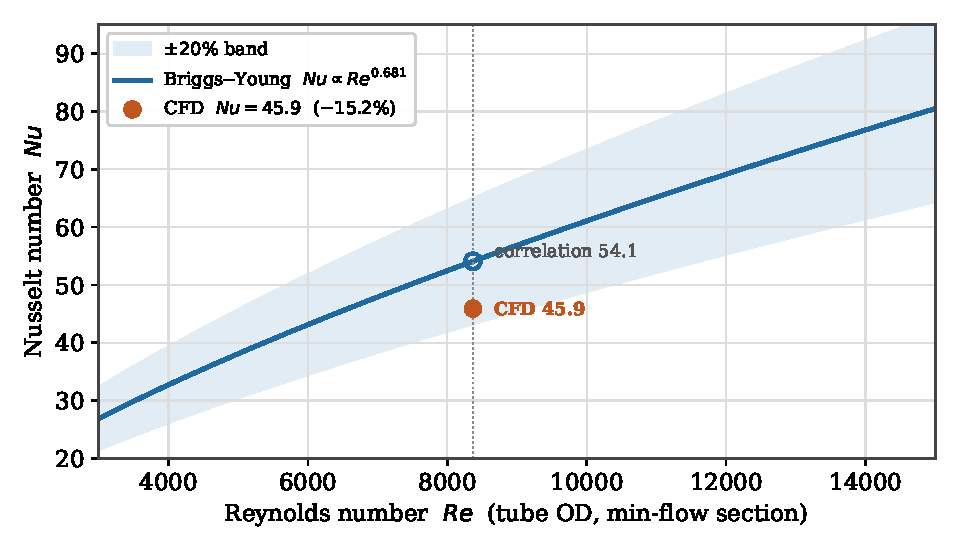
\includegraphics[width=0.78\linewidth]{fig_cfd_validation.pdf}
\caption{Single-point CFD validation of the air-side Nusselt number against the Briggs--Young correlation. The CFD
point ($Nu=45.9$) sits inside the $\pm20\%$ band, $15.2\%$ below the correlation --- close agreement for a
first-principles solve, certifying the $Nu(Re)$ law used across the operating range.}\label{fig:cfd}
\end{figure}

\begin{table}[h]\centering\small
\caption{Results summary. Each model draft removes one assumption; the penalty at \SI{55}{\celsius} converges.}\label{tab:res}
\begin{tabular}{@{}llcc@{}}
\toprule
Model & Refinement over previous & Penalty @ \SI{55}{\celsius} & Slope (\SIrange{25}{45}{\celsius})\\
\midrule
v1 & air-standard cycle, fixed firing temp.\ (conservative) & $-17.7\%$ & \SI{0.60}{\%/\celsius}\\
v1.5 & $\varepsilon$--NTU sized heat exchangers, floating TIT & $-8.8\%$ & \SI{0.15}{\%/\celsius}\\
v2 & + CFD-validated air-side law $UA\propto\dot m^{0.454}$ & $\mathbf{-8.7\%}$ & \SI{0.15}{\%/\celsius}\\
\midrule
\multicolumn{4}{@{}l}{\emph{CFD validation:}\quad $Nu=45.9$ vs.\ $54.1$ (Briggs--Young) $=-15.2\%$ \; \textbf{[validated]};
\; friction $+489\%$ [not used]}\\
\bottomrule
\end{tabular}
\end{table}

\section{Conclusion}
The desert thermal penalty for an \mbox{eVinci}-class open-air Brayton microreactor is real and large: net electric
output falls by \SIrange{9}{18}{\percent} between \SI{25}{} and \SI{55}{\celsius}, several times the Carnot-only
limit, driven by compressor-inlet thermodynamics rather than the heat-rejection hardware. A validated OpenFOAM
air-side setup confirmed the heat-exchanger law and showed the result is insensitive to it. The deliverable is a
quantitatively defensible, per-site derating band --- the physics-grounded interface that replaces the heuristic
``climate'' criterion in the Phase-2 siting platform.

\section{Key terms in plain language}
{\small\renewcommand{\arraystretch}{1.3}
\noindent\begin{tabular}{@{}p{0.25\linewidth}p{0.69\linewidth}@{}}
\toprule
\textbf{Term} & \textbf{In plain language, with an everyday example}\\
\midrule
Open-air Brayton cycle & A ground-based jet engine: it draws in outside air, squeezes it, heats it, and lets it spin a turbine, then blows the air back out. ``Open'' means it breathes the surrounding air instead of recycling a sealed gas.\\
Recuperator & A heat-recycler: the turbine's hot exhaust pre-warms the incoming air before the reactor, so less reactor heat is needed --- like exhaling into a scarf so your next breath in is already warmer.\\
Compressor-inlet temperature & The temperature of the engine's ``first breath''. In the desert this is the hot outside air, and hot air is thinner --- the same reason cars and aircraft lose power on hot days or at altitude.\\
Firing (turbine-inlet) temperature & How hot the gas is when it reaches the turbine blades: hotter gives more power, but it is capped by what the metal and heat pipes can survive --- like an oven's maximum setting.\\
Mass flow ($\dot m$) & Kilograms of air passing through each second, like litres-per-second through a pipe. Hot, thin air packs fewer kilograms per second, so less power.\\
Carnot ceiling & The best efficiency physics allows between a hot and a cold temperature --- a hard limit no engine can beat. A hotter ``cold side'' (desert air) lowers the ceiling.\\
Effectiveness ($\varepsilon$) & How close a heat exchanger gets to moving the most heat it possibly could; $\varepsilon=0.9$ means it captures 90\,\% of that maximum.\\
NTU & A heat exchanger's ``size'' relative to the flow it must heat --- a bigger car radiator has a higher NTU and moves more heat.\\
CFD & A computer experiment: the air space is chopped into millions of tiny cells and the physics solved in each --- a very detailed ``wind tunnel on a computer''.\\
Nusselt number ($Nu$) & A cooling score --- how much better moving air removes heat than still air. $Nu=46$ means the airflow removes heat about 46 times better than a stagnant layer.\\
Reynolds number ($Re$) & Whether the flow is smooth or turbulent: low is smooth like slow honey, high is churning like river rapids. Turbulent flow grabs heat better.\\
Buckingham-$\pi$ theorem & A maths shortcut that collapses many variables into a few ratios, so one small test stands in for many cases --- like a recipe that depends only on ingredient \emph{ratios} and so scales to any batch size.\\
Log-mean temp.\ difference & The correct average temperature gap between the hot wall and the warming air --- a special average, because the gap shrinks as the air heats up along the tube.\\
Briggs--Young correlation & The ``textbook answer'': a published formula from decades of lab experiments on finned tubes, used here to check the simulation.\\
\bottomrule
\end{tabular}\par}

\vspace{2pt}\noindent\rule{\linewidth}{0.4pt}
{\footnotesize\noindent Sources: \texttt{cycle\_model/derating\_v1.py}, \texttt{hx\_entu\_v1\_5.py},
\texttt{cfd/} (OpenFOAM ESI~2406); reference facts from IAEA ARIS~2024. Full rationale in
\texttt{DECISIONS\_LOG.md} (D10--D12) and \texttt{spec/A1\_reference\_spec\_sheet.md}.}

\end{document}
